%%%%%%%%%%%%%%%%%%%%%%%%%%%%%%%%%%%%%%%%
%% MCM/ICM LaTeX Template %%
%% 2022 MCM/ICM           %%
%%%%%%%%%%%%%%%%%%%%%%%%%%%%%%%%%%%%%%%%
\documentclass[12pt]{article}
\usepackage{geometry}
\geometry{left=1in,right=1in,top=1in,bottom=0.9in}

%%%%%%%%%%%%%%%%%%%%%%%%%%%%%%%%%%%%%%%%
% Replace ABCDEF in the next line with your chosen problem
% and replace 1111111 with your Team Control Number
\newcommand{\Problem}{A}
\newcommand{\Team}{mby}
%%%%%%%%%%%%%%%%%%%%%%%%%%%%%%%%%%%%%%%%

\usepackage{newtxtext}
\usepackage{amsmath,amssymb,amsthm}
\usepackage{newtxmath} % must come after amsXXX

\usepackage{ctex}    %调用中文宏包
\usepackage{cite}
\usepackage{graphicx}%图片头文件
\usepackage{xcolor}
\usepackage{fancyhdr}
\usepackage{float}
\usepackage{booktabs}
\usepackage{lastpage}
\usepackage{multirow}
\usepackage{caption}

\usepackage{diagbox}
\usepackage{listings}
\usepackage{fontspec}
\usepackage{verbatim}
\usepackage{float} %指定图片位置
%\usepackage{subfigure}%并排子图 共享标题 有子标题
\usepackage{subcaption}
\usepackage{makecell}
%\usepackage{indentfirst}
\lhead{0R2022- \Team}
\rhead{}
\cfoot{}

\newtheorem{theorem}{Theorem}
\newtheorem{corollary}[theorem]{Corollary}
\newtheorem{lemma}[theorem]{Lemma}
\newtheorem{definition}{Definition}
%\pagestyle{type} 
\begin{document}
\graphicspath{{images}}  % Place your graphic files in the same directory as your main document
\DeclareGraphicsExtensions{.pdf, .jpg, .tif, .png, .webp}
\thispagestyle{empty}
\vspace*{-16ex}
%\centerline{\begin{tabular}{*3{c}}

%%%%%%%%%%% Begin Summary %%%%%%%%%%%
% Enter your summary here replacing the (red) text
% Replace the text from here ...
%\begin{center}
    \section*{Summary}
\end{center}



\section*{Keywords} %%%小写

% to here
%%%%%%%%%%% End Summary %%%%%%%%%%%
\setlength{\headheight}{15pt}
%\clearpage
%%%%%%%%%%%%%%%%设置目录%%%%%%%%%%%%%%
\pagestyle{fancy}
% Uncomment the next line to generate a Table of Contents
%\tableofcontents 
\tableofcontents
\setcounter{page}{1}
\rhead{Page \thepage\ of \pageref{LastPage}}
%%%%%%%%%%%%%%%%%%%%%%%%%%%%%%

%%%%%%%%%%%%%%%%开始正文%%%%%%%%%%%%%%
\newpage
\section{研究背景}
\subsection{背景说明}
在校园面积较大的高校,师生通常会使用代步工具包括自行车、电瓶车、电动滑板等进行校园内通勤。电瓶车、电动滑板需要定期进行充电,而将电瓶带入宿舍或是从宿舍拉电线的充电行为有极大的安全隐患,被高校明令禁止。为解决师生充电困难问题,校方通常会在校园开阔地带建设固定充电桩。\\
\indent 以成电清水河校区为例,经调查校园现有15个充电点位,每个充电点位可同时容纳24辆电动自行车充电。分布情况如图所示:
\begin{figure}[H]
    \centering
    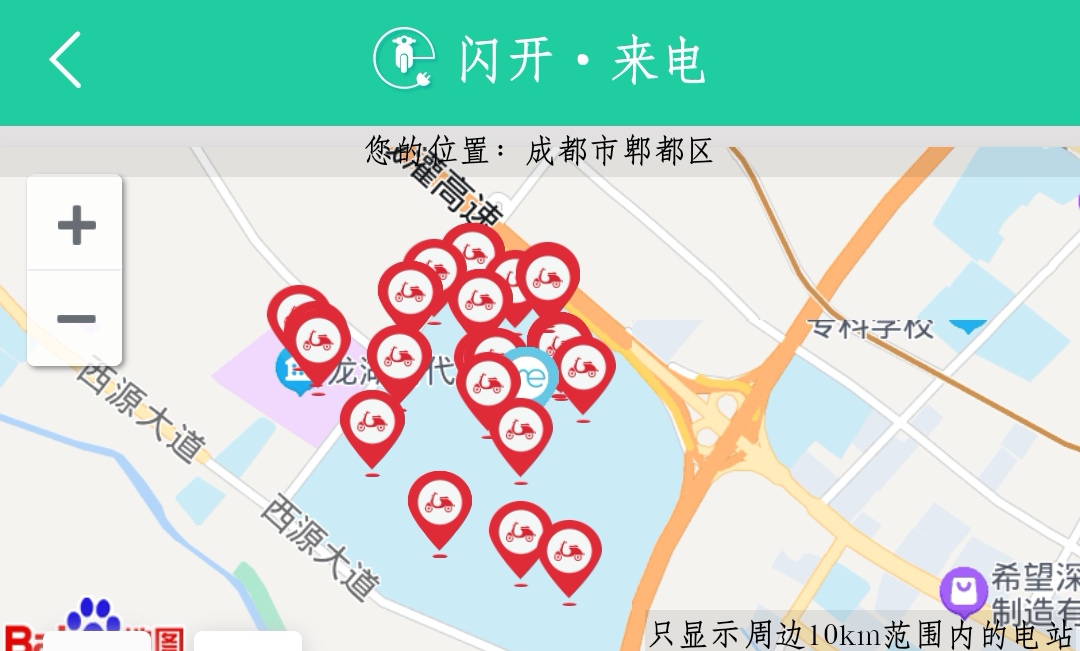
\includegraphics[width=0.6\textwidth]{pic1.jpg}
    %\caption{自卸车卸货的两个过程}
    \caption{闪开来电校园充电桩分布}
\end{figure}
但是在校园论坛中我们发现同学们对于设置地点与充电口数目不合理的抱怨。比如,充电桩离自己常去的地方过远,来往于充电路途非常花时间;充电桩数目过少,不易寻找到空闲位置……\\
\indent 对于上述问题,我们认为对于充电桩建设点位进行规划可以减缓同学的抱怨。什么地方可以建设充电桩,在什么地方建设充电桩会更好。\\
\indent 我们对校园内环境进行了调研,我们归纳出包括但不限于现有充电桩的30个可建设充电桩位置.(\textit{基本要求:空余面积不小于15$m^2$、附近可接入电源、满足一定人流量})
\subsection{研究目标}
那么在固定充电桩设置地点与充电口数目的情况下,校方对于充电桩的选址是否最优,如果不是最优选址,那么最优选址应该被定在哪里。以及在每一个充电桩应该预留多少个充电口引起了我们的好奇,我们希望能通过运筹学的方式得到问题的解答。








\section{模型假设与分析}
\begin{enumerate}
    \item 统计对象限制在成电清水河校区的研究生\\
    $\hookrightarrow $\textit{分析:本科生活动范围集中于校园南侧区域、较少有同学购买电动自行车;研究生教研室分布距离宿舍区普遍较远且自身财力更能支持其购买电动自行车,研究生群体中拥有电动车比例远高于本科生。} 
  
    \item 模型参考运输问题进行建立。\\
    $\hookrightarrow $\textit{分析:电动车充电需要从骑者地点运输至充电桩进行充电,可将双方看作产地与销地,费用以路程代替。至于‘产量’‘销量’的大小关系,可将其假设大小相同(免除虚拟地的假设).}\textbf{最终计算结果用以衡量比例大小关系而非绝对数值关系。} 

\end{enumerate}
\section{数据收集与分析}
\subsection{需要数据与预估收集方式}
\begin{itemize}
    \item [\textbf{$\bullet $}] 确定校园满足充电桩建设的地点地点位置级数量、 校方目前在其中地建设了充电桩的地点位置级数量、所有充电桩建设地点拥有充电口总数$\implies $\textit{自行在校园内排查}
    \item [\textbf{$\bullet $}] 校内拥有需充电设备的师生最常去的几个地点地区$\implies $\textit{问卷调查}
    \item  [\textbf{$\bullet $}]以及点与点间的距离进行统计$\implies $\textit{自行在校园内排查}
    \item [\textbf{$\bullet $}]师生的充电偏好(充电时间/充电时长/周充电频率等)$\implies $\textit{问卷调查}
\end{itemize}
\subsection{数据呈现}
\begin{figure}[H]
	\centering
	\subcaptionbox{可行的30处充电桩建设点}{
		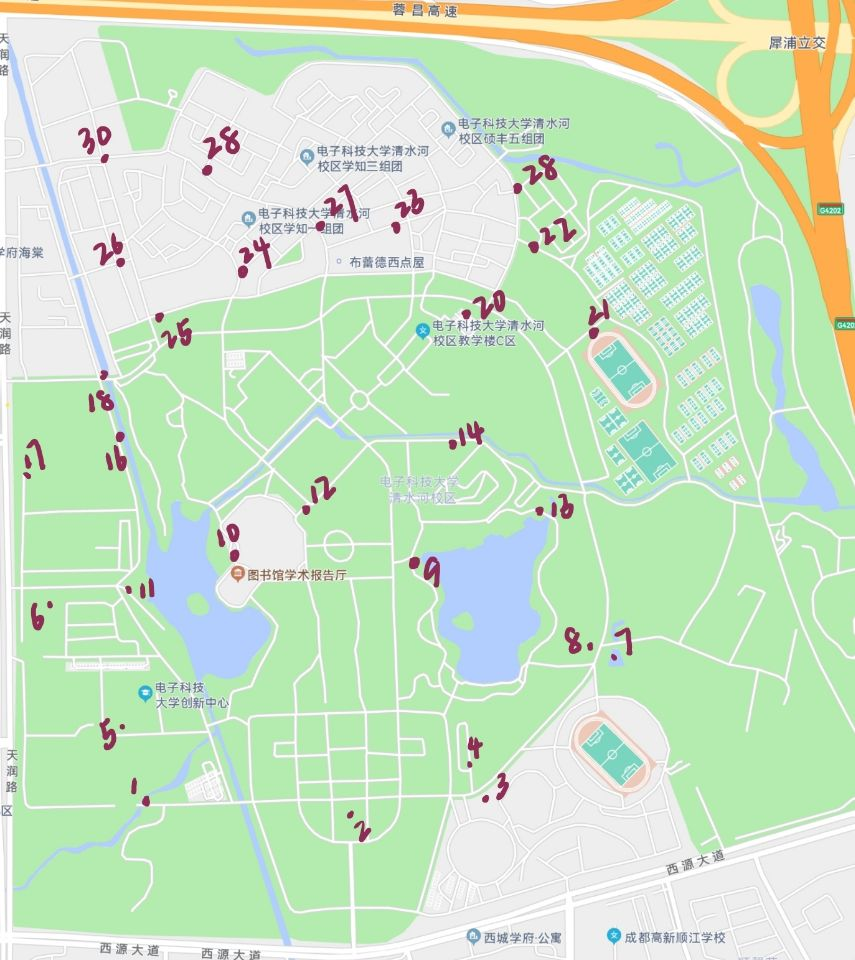
\includegraphics[width=5.5cm]{pic2.jpg}		
	}
	%\hfill % 是为了让多幅图在一行均匀分布(不加的效果是都挤在中间)
	\subcaptionbox{研究生通常活动区域}{
		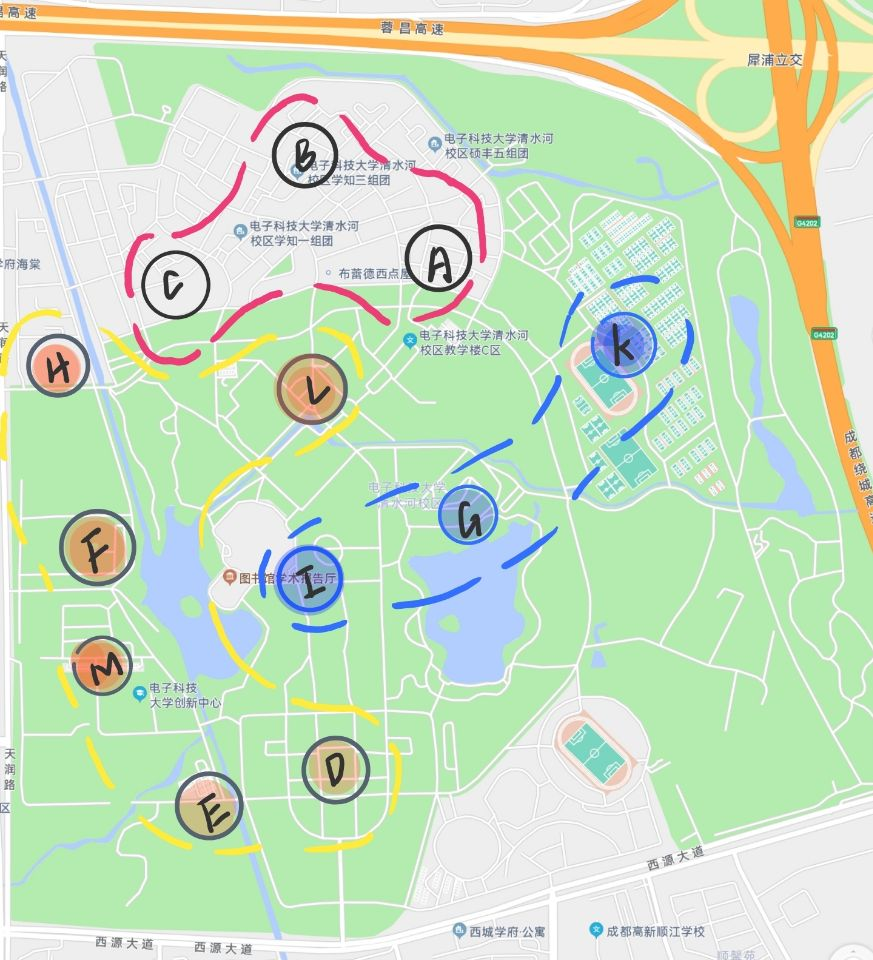
\includegraphics[width=5.5cm]{pic3.jpg}	
	}
	
	\label{functionrelationship}
\end{figure}

\begin{table}[H]\small
	\centering
	\caption{通常活动区域\textit{常驻地}与充电桩\textit{目的地}间距离}
	%\label{频率型、强度型和相对比型指标}也可以用这个
	\begin{tabular}{c|p{0.60cm}<{\centering}|p{0.6cm}<{\centering}|p{0.6cm}<{\centering}|p{0.6cm}<{\centering}|p{0.6cm}<{\centering}|p{0.6cm}<{\centering}|p{0.6cm}<{\centering}|p{0.6cm}<{\centering}|p{0.6cm}<{\centering}|p{0.6cm}<{\centering}|p{0.6cm}<{\centering}|p{0.54cm}<{\centering}}
		\toprule[2pt]  %添加表格头部粗线
		\diagbox{\footnotesize {目的地$j$}}{\footnotesize {距离($m$)}}{\footnotesize {常驻地$i$}} &  A & B & C & D & E & F & M & L & H & I & G & K \\
		\midrule[1.75pt]  %添加表格中横线
		1 & 1900 & 1900 & 1551 & 317 & 15 & 518 & 680 & 1420 & 1304 & 797 & 751 & 2456 \\ 
        2 & 1474 & 1474 & 1474 & 0 & 233 & 714 & 363 & 1185 & 1227 & 564 & 564 & 2030 \\ 
        3 & 1518 & 1518 & 1518 & 252 & 485 & 966 & 615 & 1418 & 1271 & 797 & 751 & 2074 \\ 
        4 & 1557 & 1557 & 1557 & 321 & 554 & 1035 & 684 & 1463 & 1310 & 807 & 838 & 2113 \\ 
        5 & 1780 & 1780 & 1431 & 456 & 223 & 473 & 102 & 1566 & 1184 & 926 & 796 & 2336 \\ 
        6 & 1379 & 1379 & 1030 & 728 & 495 & 239 & 31 & 1168 & 783 & 1136 & 986 & 1935 \\ 
        7 & 1200 & 1300 & 1300 & 652 & 885 & 1366 & 1074 & 1179 & 1053 & 878 & 541 & 1756 \\ 
        8 & 900 & 991 & 991 & 925 & 1158 & 1639 & 1347 & 882 & 744 & 538 & 201 & 1456 \\ 
        9 & 906 & 906 & 906 & 564 & 797 & 1278 & 986 & 1155 & 659 & 121 & 21 & 1462 \\ 
        10 & 914 & 914 & 856 & 702 & 935 & 1416 & 1124 & 439 & 609 & 31 & 210 & 1470 \\ 
        11 & 1300 & 1300 & 951 & 714 & 481 & 11 & 1136 & 762 & 704 & 1265 & 1195 & 1856 \\ 
        12 & 838 & 838 & 489 & 798 & 1031 & 1512 & 1220 & 390 & 242 & 82 & 121 & 1394 \\ 
        13 & 1000 & 1000 & 1000 & 1000 & 1233 & 1714 & 1422 & 1034 & 753 & 426 & 89 & 1556 \\ 
        14 & 848 & 848 & 848 & 1240 & 1473 & 1954 & 1662 & 882 & 601 & 426 & 89 & 1404 \\ 
        15 & 658 & 658 & 358 & 867 & 1100 & 1581 & 1289 & 178 & 111 & 212 & 242 & 1214 \\ 
        16 & 1000 & 1000 & 700 & 966 & 733 & 100 & 329 & 452 & 453 & 938 & 1326 & 1556 \\ 
        17 & 1100 & 1100 & 800 & 1103 & 870 & 100 & 379 & 452 & 553 & 938 & 1326 & 1656 \\ 
        18 & 868 & 868 & 519 & 1115 & 882 & 360 & 510 & 889 & 272 & 1375 & 1230 & 1424 \\ 
        19 & 626 & 626 & 500 & 1185 & 1418 & 882 & 1607 & 32 & 253 & 439 & 793 & 1182 \\ 
        20 & 306 & 584 & 584 & 1406 & 1639 & 1539 & 1828 & 149 & 337 & 635 & 738 & 862 \\ 
        21 & 454 & 875 & 875 & 1791 & 2024 & 1420 & 2213 & 534 & 628 & 1020 & 991 & 0 \\ 
        22 & 290 & 654 & 654 & 1621 & 1854 & 1340 & 2043 & 364 & 897 & 850 & 1082 & 231 \\ 
        23 & 200 & 350 & 350 & 1385 & 1618 & 1104 & 1807 & 128 & 593 & 614 & 707 & 756 \\ 
        24 & 572 & 572 & 133 & 1364 & 1131 & 715 & 844 & 107 & 815 & 593 & 891 & 1128 \\ 
        25 & 758 & 758 & 319 & 1478 & 1245 & 615 & 744 & 221 & 1001 & 707 & 991 & 1314 \\ 
        26 & 817 & 726 & 340 & 1572 & 1339 & 654 & 783 & 315 & 969 & 801 & 1080 & 1373 \\ 
        27 & 520 & 258 & 258 & 1223 & 1456 & 1310 & 1439 & 152 & 501 & 638 & 707 & 1076 \\ 
        28 & 329 & 469 & 719 & 1791 & 2024 & 1327 & 2213 & 534 & 712 & 1020 & 1201 & 389 \\ 
        29 & 770 & 129 & 129 & 1538 & 1771 & 1239 & 1360 & 281 & 372 & 767 & 919 & 1326 \\ 
        30 & 953 & 567 & 149 & 1730 & 1497 & 897 & 1018 & 473 & 810 & 959 & 1102 & 1509 \\ 
		\bottomrule[2pt] %添加表格底部粗线
	\end{tabular}
\end{table}
我们将学生常去的地区\textit{常驻地},做出三种分类:宿舍区(ABC),学习/教研室区(DEFMLH),休闲/其他常去区(IGK)。\\
\indent 以下表格根据问卷结果与实际学院人数、对应教研室位置做出统计:
\begin{table}[H]
    \centering
	\caption{收集问卷结果:学生常去区域的时间分配$S_{k}$}
    %\label{频率型、强度型和相对比型指标}也可以用这个
    \begin{tabular}{c|p{2cm}<{\centering}|p{3cm}<{\centering}|p{3cm}<{\centering}}
        \toprule  %添加表格头部粗线
        \diagbox{常去情况}{区域} & 宿舍区(ABC) & 学习区(DEFMLH)& 其他休闲区(IGK)  \\
        \midrule  %添加表格中横线
        时间分配 & 30\% & 60\% & 10\%\\
        
        \bottomrule %添加表格底部粗线
    \end{tabular}
\end{table}

\begin{table}[H]
    \centering
	\caption{问卷数据统计结果:宿舍区}
    \begin{tabular}{c|p{3cm}<{\centering}|p{3cm}<{\centering}|p{3cm}<{\centering}}
        \toprule  %添加表格头部粗线
        \diagbox{情况}{常驻地} & A & B& C \\
        \midrule  %添加表格中横线
        学生比例分配 & 33.33\% & 33.33\% & 33.33\%\\
        \bottomrule %添加表格底部粗线
    \end{tabular}
\end{table}
\begin{table}[H]
    \centering
	\caption{实际学院人数数据计算结果:学习区}
    \begin{tabular}{c|p{1.7cm}<{\centering}|p{1.7cm}<{\centering}|p{1.7cm}<{\centering}|p{1.7cm}<{\centering}|p{1.7cm}<{\centering}|p{1.7cm}<{\centering}}
        \toprule  %添加表格头部粗线
        \diagbox{情况}{常驻地} & D & E& F&M&L&H \\
        \midrule  %添加表格中横线
        学生比例分配 & 18.93\%&	11.27\%&	29.06\%&	12.74\%&	18.12\%&	9.87\%\\

        \bottomrule %添加表格底部粗线
    \end{tabular}
\end{table}
\begin{table}[H]
    \centering
	\caption{问卷数据统计结果:其他休闲区}
    \begin{tabular}{c|p{2cm}<{\centering}|p{3cm}<{\centering}|p{3cm}<{\centering}}
        \toprule  %添加表格头部粗线
        \diagbox{情况}{常驻地} & I & G& K \\
        \midrule  %添加表格中横线
        学生比例分配 & 50\% & 20\% & 30\%\\
        \bottomrule %添加表格底部粗线
    \end{tabular}
\end{table}
\section{符号说明}
\begin{table}[H]
\begin{center}
\caption{符号对照表}
\begin{tabular}{p{3cm}<{\centering} |c}

\toprule[1.75pt]
    符号 & 定义\\
\midrule[1pt]
    $x_{ij}$  & 从常驻地$i$分配到目的地$j$的数目    \\
    $c_{ij}$  & 从常驻地$i$分配到目的地$j$的路程成本 \\
    $Z$       & 总的电动车运输路程\\
    $a_{i}$   & 产出量\textit{(从常驻地$i$出发的电动车数量)}\\
    $b_{j}$   & 可接受量\textit{(目的地$j$可接受的电动车数量)}\\
    $Q$       & 各点位电动车最大容纳量\textit{(沿用现成数据24作为计算值)}\\
    $S_{k}$   &各类型区域时间分配比例\\
\bottomrule[1.75pt]

\end{tabular}

\end{center}
\end{table}


\input{model3}
\input{part2}
\input{part3}
\input{part4}
\section{建立模型}
\indent 模型如下:\\
\begin{equation}
    min Z=\sum_{k = 1}^{3}S_{k}(\sum_{i = 1} \sum_{j = 1}^{30}x_{ij}c_{ij} )    
\end{equation}
\begin{equation}
    s.t.\left\{
        \begin{aligned}
        \sum_{i}a_{i} & =  \sum_{j = 1}^{30}b_{j}\\
        \sum_{j = 1}x_{ij} & =  b_{j}\eqslantless Q\\
        \sum_{i = 1}x_{ij} &  =  a_{i} \\
        x_{ij}& \geqslant  0\\
        \end{aligned}
        \right.
\end{equation}
\section{模型求解}
以学生常去的地区为区分,分别利用已知数据进行求解。使用EXCLE-solver。 由于‘可变单元格过多’,所以先将三类区域运输分配分别求值,再进行整合。\\
\indent 以300为电动自行车运输总数,进行后续计算。
\subsection{分区域-充电桩设置}
\begin{figure}[H]
    \centering
    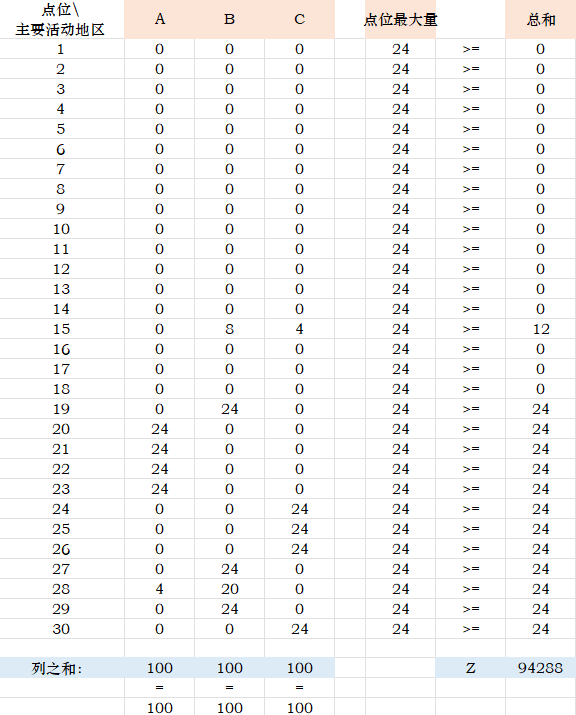
\includegraphics[width=0.5\textwidth]{pic.png}
    %\caption{自卸车卸货的两个过程}
    \caption{宿舍区-充电桩设置}
\end{figure}
\begin{figure}[H]
    \centering
    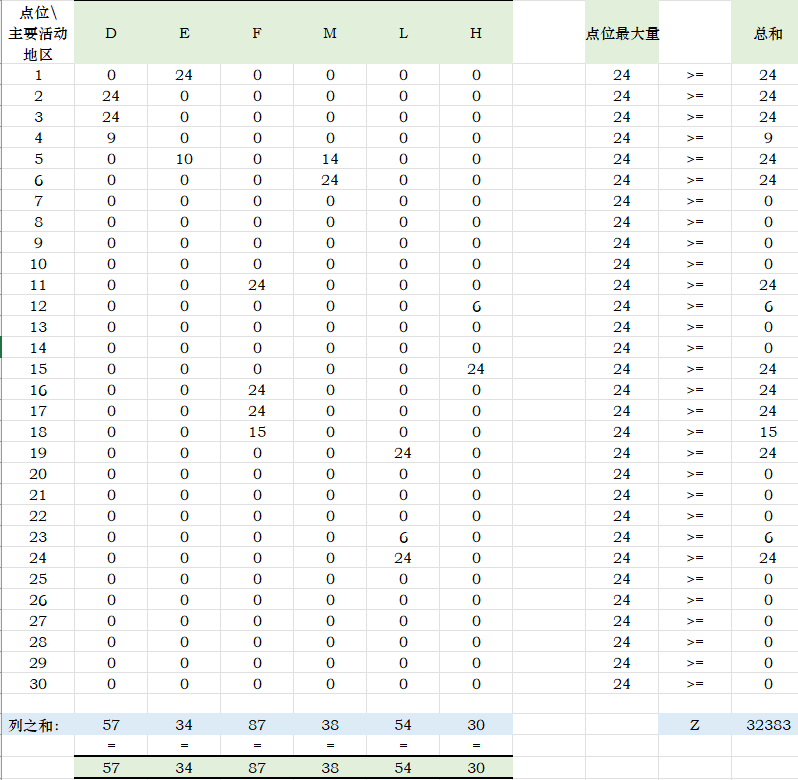
\includegraphics[width=0.5\textwidth]{pic5.png}
    %\caption{自卸车卸货的两个过程}
    \caption{学习区-充电桩设置}
\end{figure}
\begin{figure}[H]
    \centering
    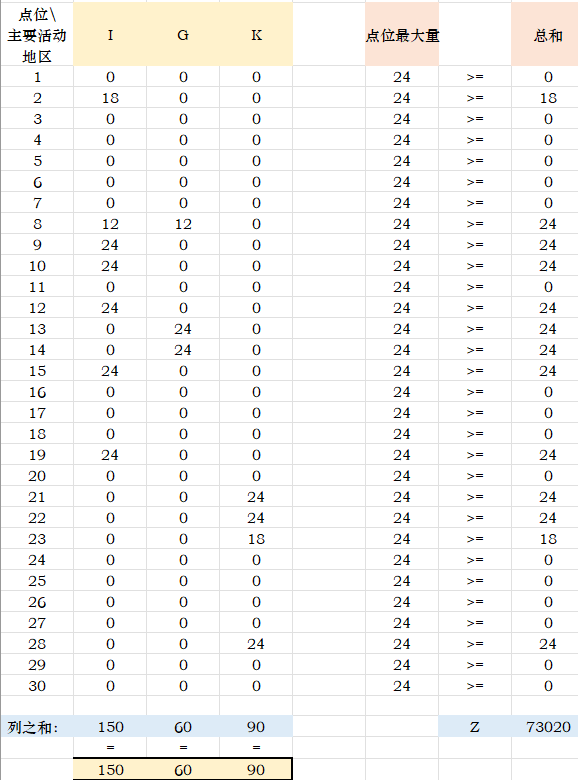
\includegraphics[width=0.4\textwidth]{pic6.png}
    %\caption{自卸车卸货的两个过程}
    \caption{其他休闲区-充电桩设置}
\end{figure}
\subsection{求解数据合并}
\begin{table}[H]
    \centering
	\caption{求解各目的地$i$可容纳电动车数目}
    \begin{tabular}{cp{3cm}<{\centering}||cp{3cm}<{\centering}||cp{3cm}<{\centering}}
        \toprule  %添加表格头部粗线
        目的地$j$ & 所需充电口数目 &  目的地$j$&所需充电口数目 & 目的地$j$&所需充电口数目\\
        \midrule  %添加表格中横线
        1 & 14  & 11 & 14 & 21 & 10 \\ 
        2 & 16  & 12 & 6  & 22 & 10 \\ 
        3 & 14  & 13 & 2  & 23 & 13 \\ 
        4 & 5  & 14 & 2  & 24 & 22 \\ 
        5 & 14  & 15 & 20  & 25 & 7 \\ 
        6 & 14  & 16 & 14  & 26 & 7 \\ 
        7 & 0  & 17 & 14  & 27 & 7 \\ 
        8 & 2  & 18 & 9  & 28 & 10 \\ 
        9 & 2  & 19 & 24  & 29 & 7 \\ 
        10 & 2  & 20 & 7  & 30 & 7 \\ 
        \bottomrule %添加表格底部粗线
    \end{tabular}
\end{table}
\begin{table}[H]
    \centering
	\caption{\textbf{排序后}求解各目的地$i$可容纳电动车数目}
    \begin{tabular}{cp{3cm}<{\centering}||cp{3cm}<{\centering}||cp{3cm}<{\centering}}
        \toprule  %添加表格头部粗线
        目的地$j$ & 所需充电口数目 &  目的地$j$&所需充电口数目 & 目的地$j$&所需充电口数目\\
        \midrule  %添加表格中横线
        19 & 24 & 17 & 14  & 29 & 7 \\ 
        24 & 22  & 23 & 13  & 30 & 7 \\ 
        15 & 20  & 21 & 10  & 12 & 6 \\ 
        2 & 16  & 22 & 10  & 4 & 5 \\ 
        1 & 14  & 28 & 10  & 8 & 2 \\ 
        3 & 14  & 18 & 9  & 9 & 2 \\ 
        5 & 14  & 20 & 7  & 10 & 2 \\ 
        6 & 14  & 25 & 7 &  13 & 2 \\ 
        11 & 14  & 26 & 7 &  14 & 2 \\ 
        16 & 14  & 27 & 7 &  7 & 0 \\ 
        \bottomrule %添加表格底部粗线
    \end{tabular}
\end{table}

\section{结论}
由上表8可知,排在表左上侧目的地$i$更被需要,而右下角目的地$i$反之。\\
\indent 那么如果仍然校园内仍保留15处充电桩建设点位,且每点位最多可同时容纳24量车进行充电,那么18、20、25、26……10,13,14,7这15个点位的充电桩不应继续使用或是被新建设.
\begin{figure}[H]
    \centering
    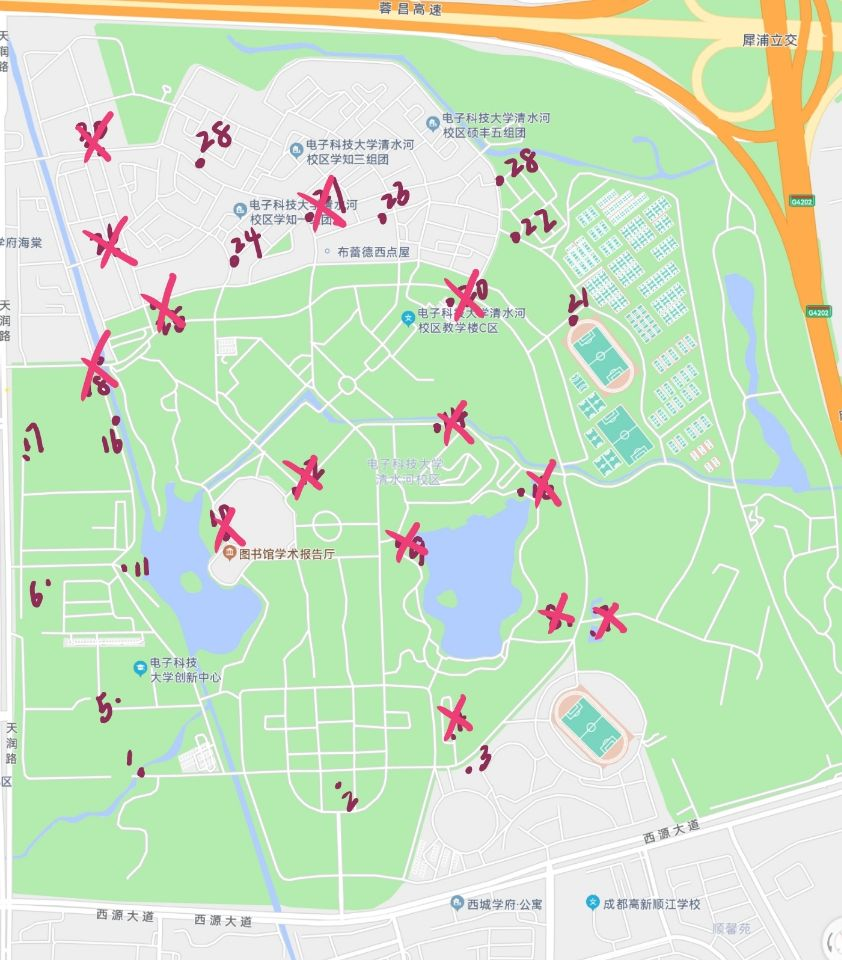
\includegraphics[width=0.4\textwidth]{pic7.jpg}
    %\caption{自卸车卸货的两个过程}
    \caption{取消与保留充电桩建设点位}
\end{figure}
\begin{figure}[H]
    \centering
    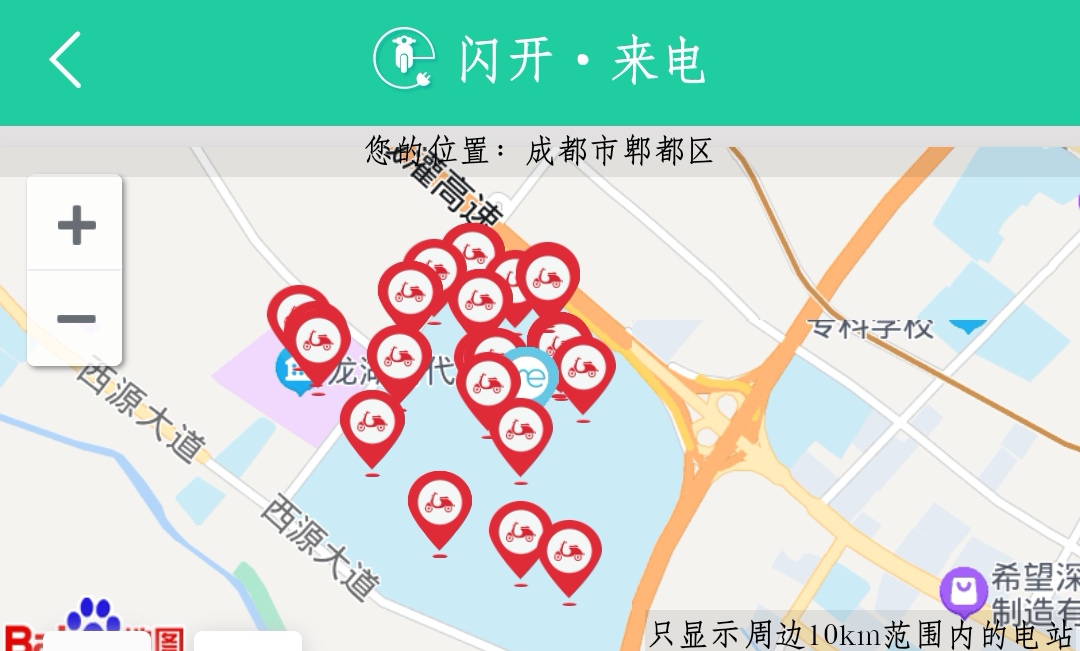
\includegraphics[width=0.6\textwidth]{pic1.jpg}
    %\caption{自卸车卸货的两个过程}
    \caption{与现有校园充电桩分布进行对比}
\end{figure}
与现有校园充电桩分布进行对比分析有:现有充电桩再商业街学生活动中心处布点过分密集,但在西门-西二门附近学生需求量较大区域布点明显不足。同时,在南门体育场附近布点冗余可以取消,其他位置布点合理与计算结果基本重合。
\section{附录}
\indent 原始收集数据可见:$base\_data.xlsx$\\
\indent 计算过程可见:$caculate\_data.xlsx$
%\bibliographystyle{plain}
%\bibliography{ref}
%\section*{附录}
原始收集数据可见\textit{:base_data.xlsx}\\
计算过程可见\textit{:caculate_data.xlsx}
%%%%%%%%%%%%%%%%%%%%%%%%%%%%%%
\end{document}
\end